\section{External Interface Requirements}
\subsection{User Interfaces}
The following mockups provide a model of graphic interface that will show our program. \\
We will create a user interface that will be user friendly in order to be easy to use also from non-technical users. \\
We list the following mockups that cover all application main aspects: \\




\begin{figure}[!tbp]
  \caption{Login: Users already registered signes in with their credential}
  \label{fig:Login}
  \centering
  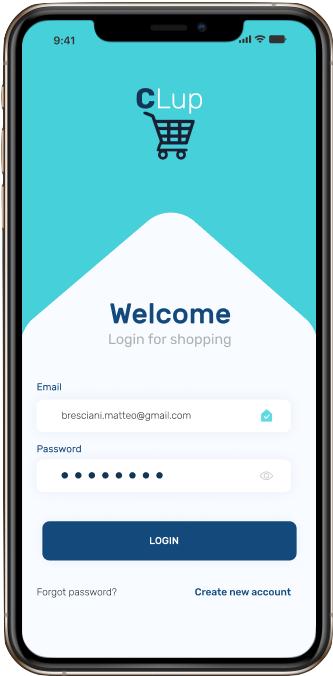
\includegraphics[scale=0.35]{images/mockup/login.png}

\end{figure}

\begin{figure}[!tbp]
  \caption{Login: Users already registered signes in with their credential}
  \label{fig:Login}
  \centering
 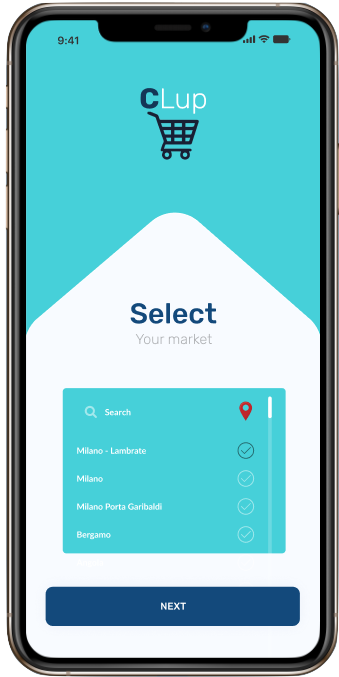
\includegraphics[scale=0.35]{images/mockup/select2.png}

\end{figure}







\begin{figure}[!tbp]
  \centering
  \subfloat[Page 1.]{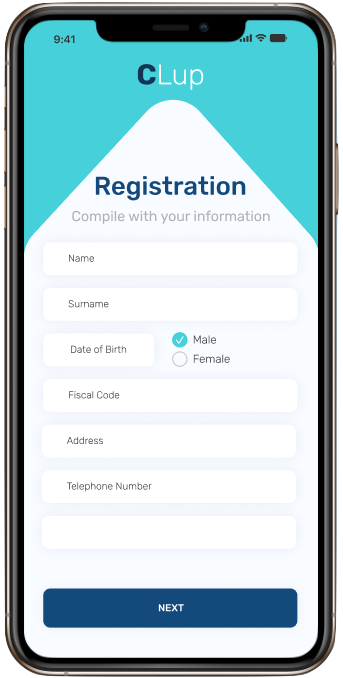
\includegraphics[scale=0.35]{images/mockup/reg1.png}\label{fig:f1}}
  \hfill
  \subfloat[Page 2]{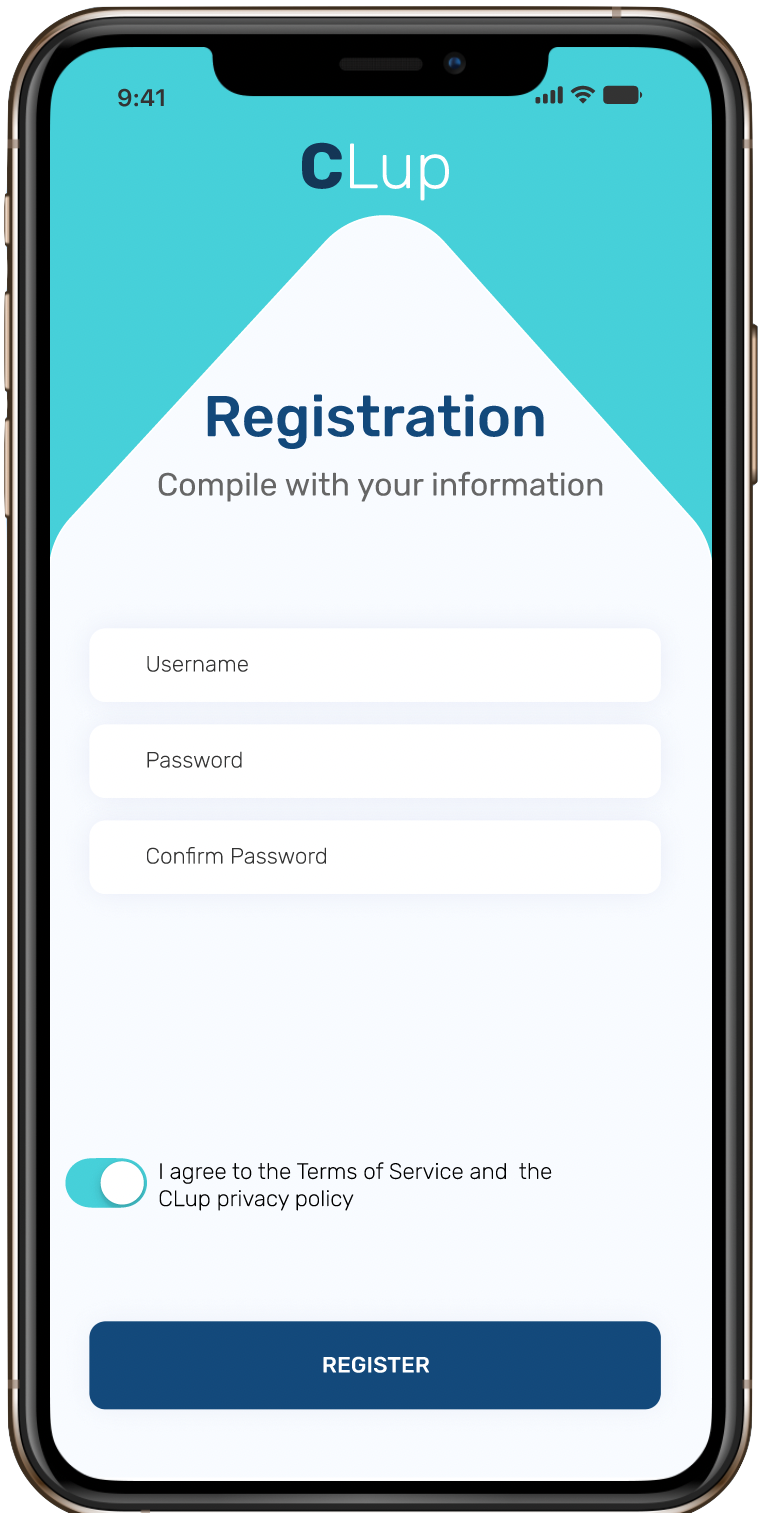
\includegraphics[scale=0.35]{images/mockup/reg2.png}\label{fig:f2}}
  \caption{Registration: Users not registered can register himself putting his own data, e-mail and password. In addition Users have to accepts the Term of Service and the CLup privacy policy to proceed.}
\end{figure}




\begin{figure}[!tbp]
  \caption{Login: Users already registered signes in with their credential}
  \label{fig:Login}
  \centering
  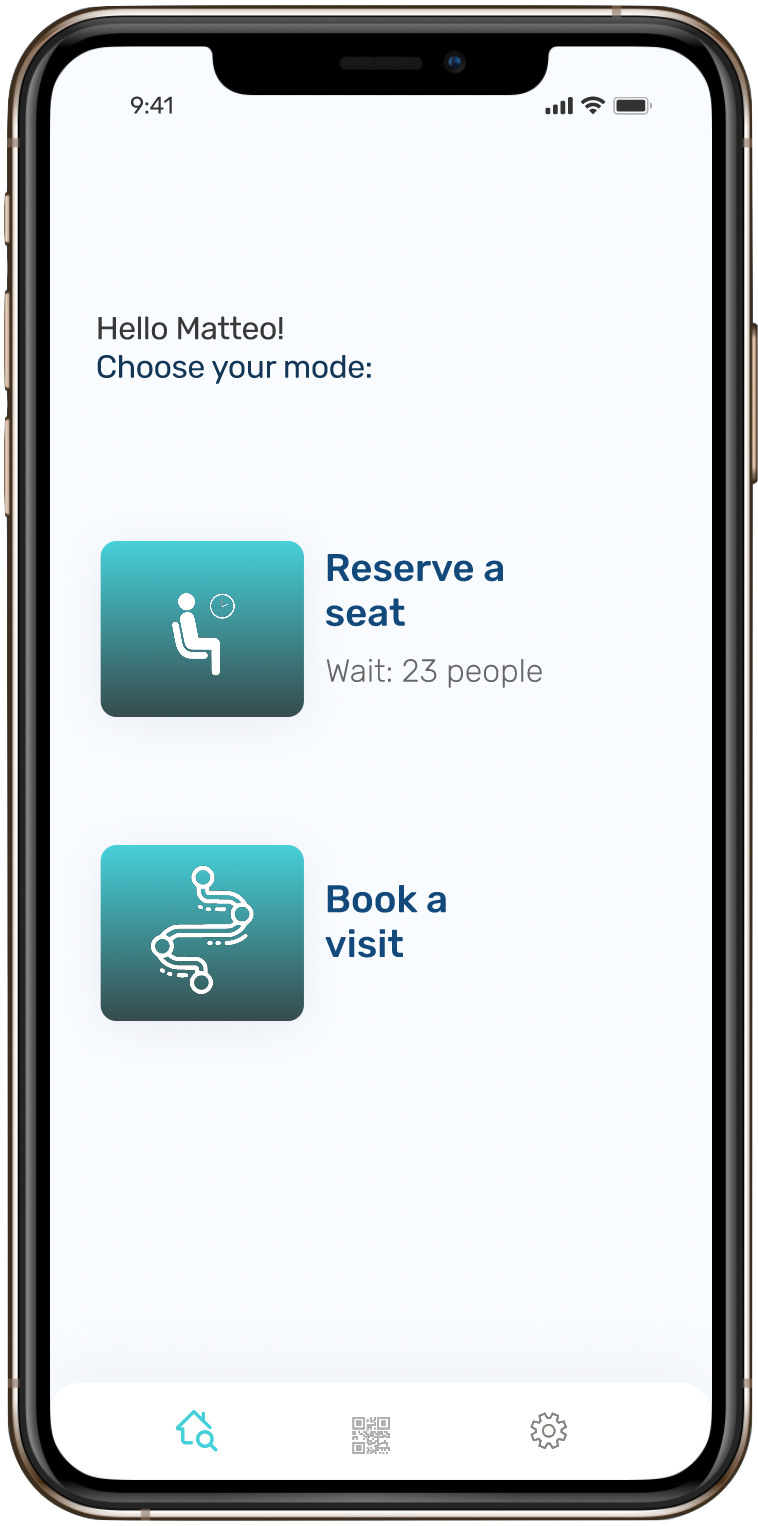
\includegraphics[scale=0.35]{images/mockup/home1.png}

\end{figure}


\begin{figure}[!tbp]
  \caption{Login: Users already registered signes in with their credential}
  \label{fig:Login}
  \centering
  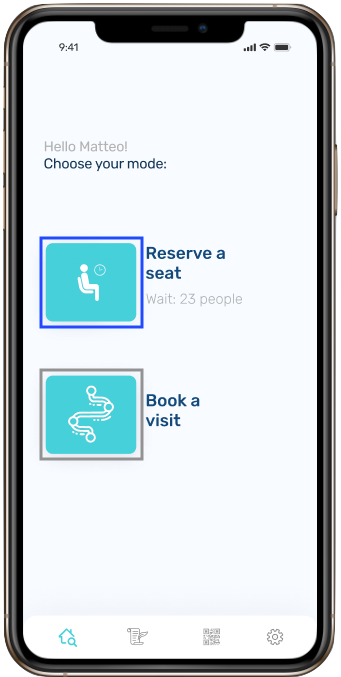
\includegraphics[scale=0.35]{images/mockup/home_options.png}

\end{figure}


\begin{figure}[ht!]
     \begin{center}
%
        \subfloat[Caption of First Figure]{%
            \label{fig:first}
            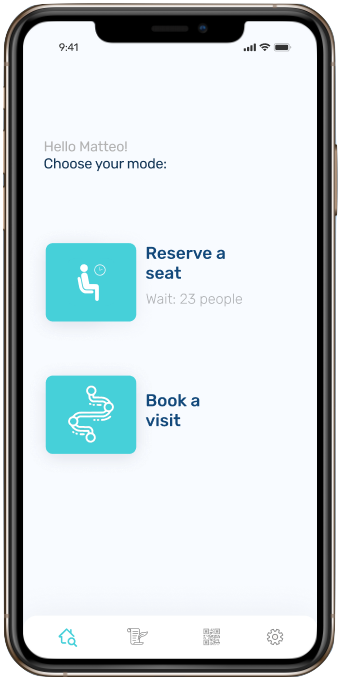
\includegraphics[scale=0.35]{images/mockup/reserve1.png}
        }%
        \subfloat[Caption of Second Figure]{%
           \label{fig:second}
           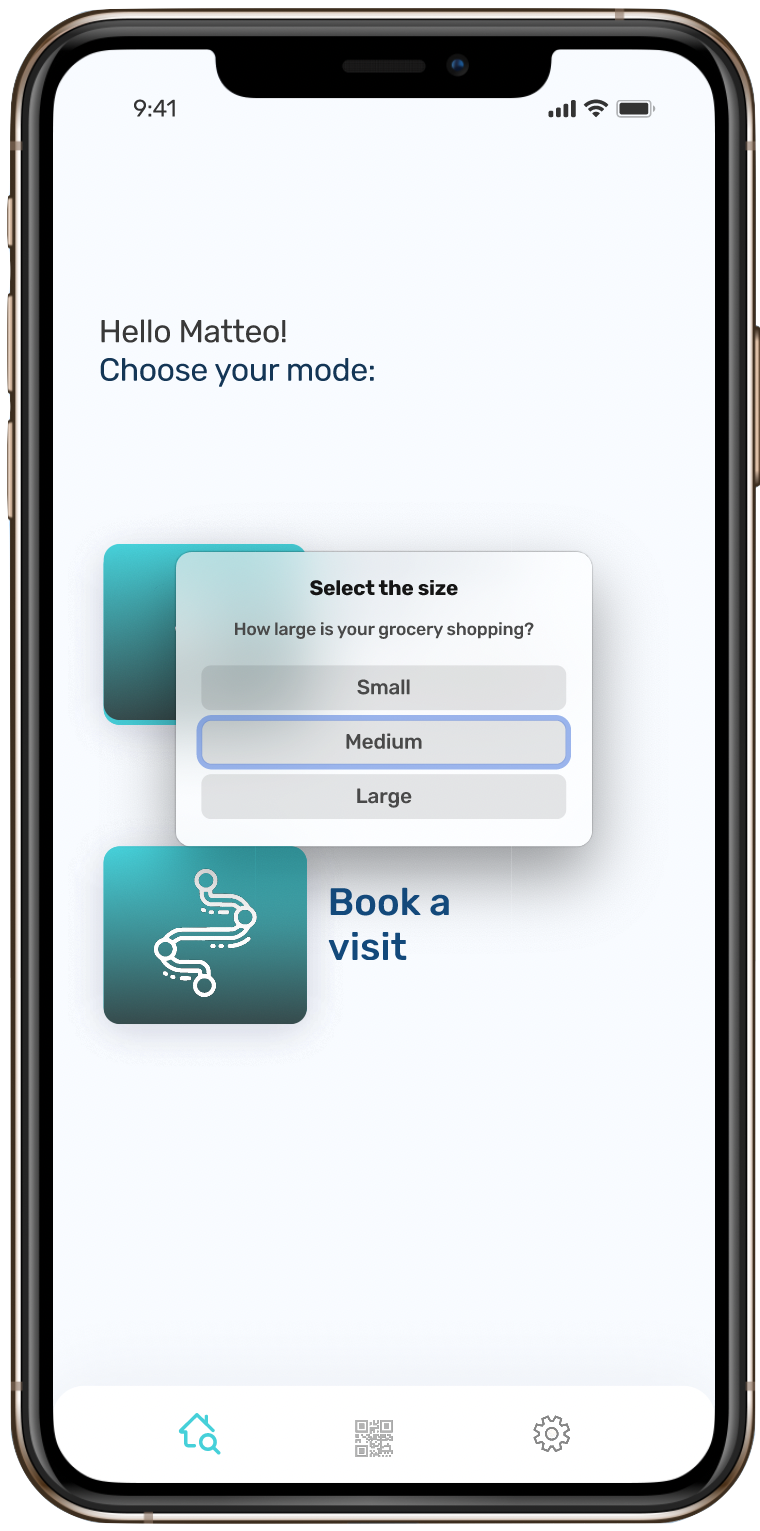
\includegraphics[scale=0.35]{images/mockup/reservation_size.png}
        }\\ %  ------- End of the first row ----------------------%
        \subfloat[Caption of Third Figure]{%
            \label{fig:third}
            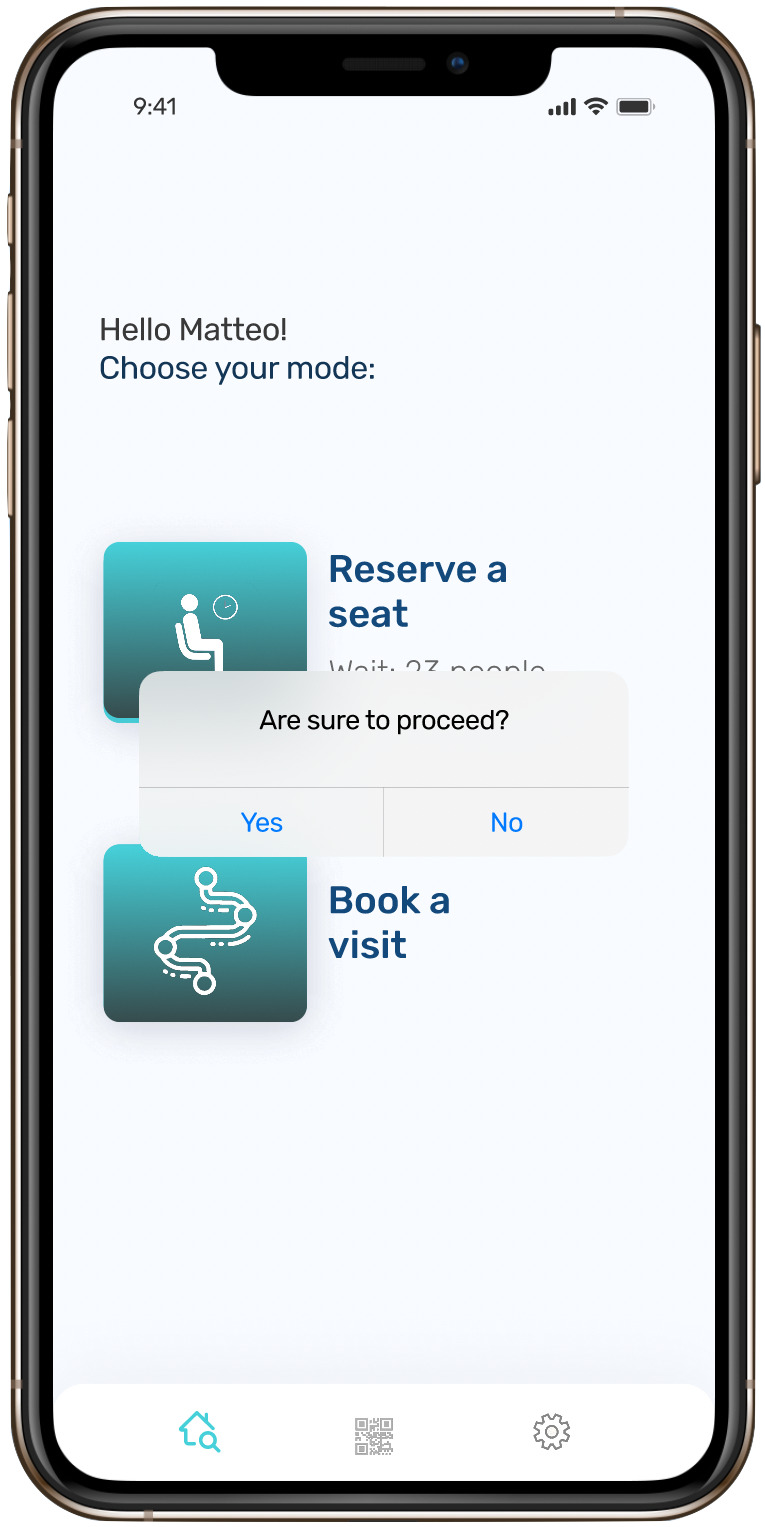
\includegraphics[scale=0.35]{images/mockup/reserve2.png}
        }%
        \subfloat[Caption of Fourth Figure]{%
            \label{fig:fourth}
            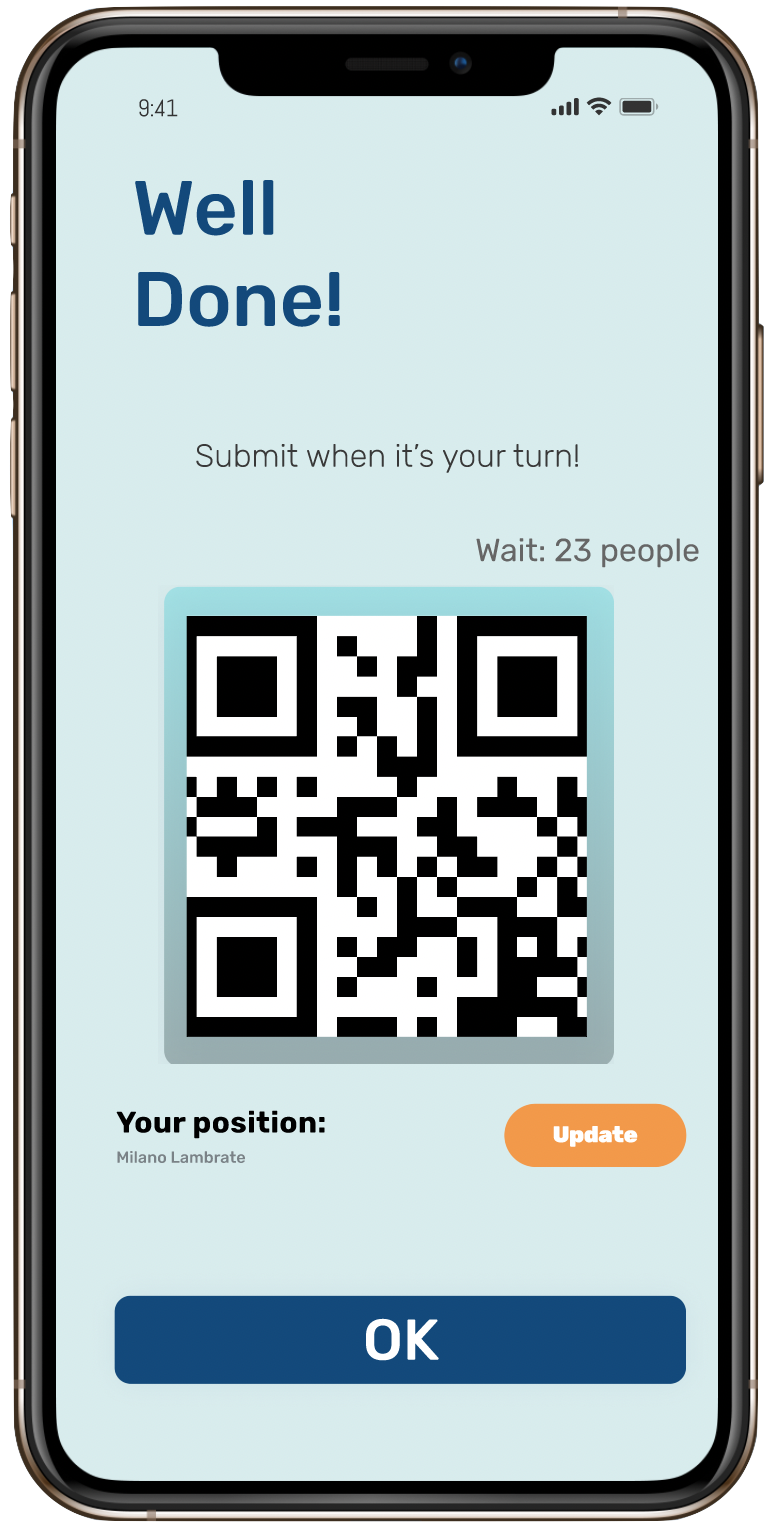
\includegraphics[scale=0.35]{images/mockup/qrcode_reservation_done.png}
        }%
%
    \end{center}
    \caption{%
        The l-o-n-g caption for all the subfigures
        (FirstFigure through FourthFigure) goes here.
     }%
   \label{fig:subfigures}
\end{figure}

\begin{figure}[ht!]
     \begin{center}
%
        \subfloat[Caption of First Figure]{%
            \label{fig:first}
            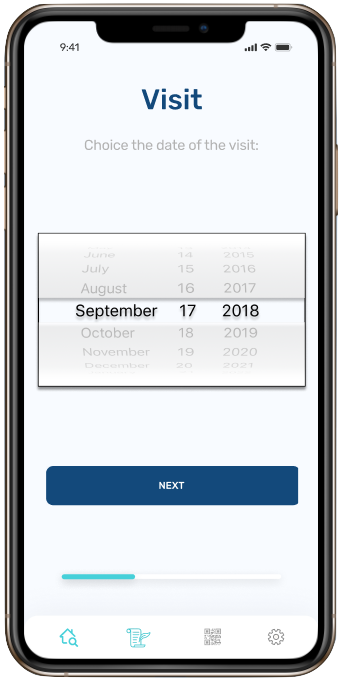
\includegraphics[scale=0.35]{images/mockup/visit1.png}
        }%
        \subfloat[Caption of Second Figure]{%
           \label{fig:second}
           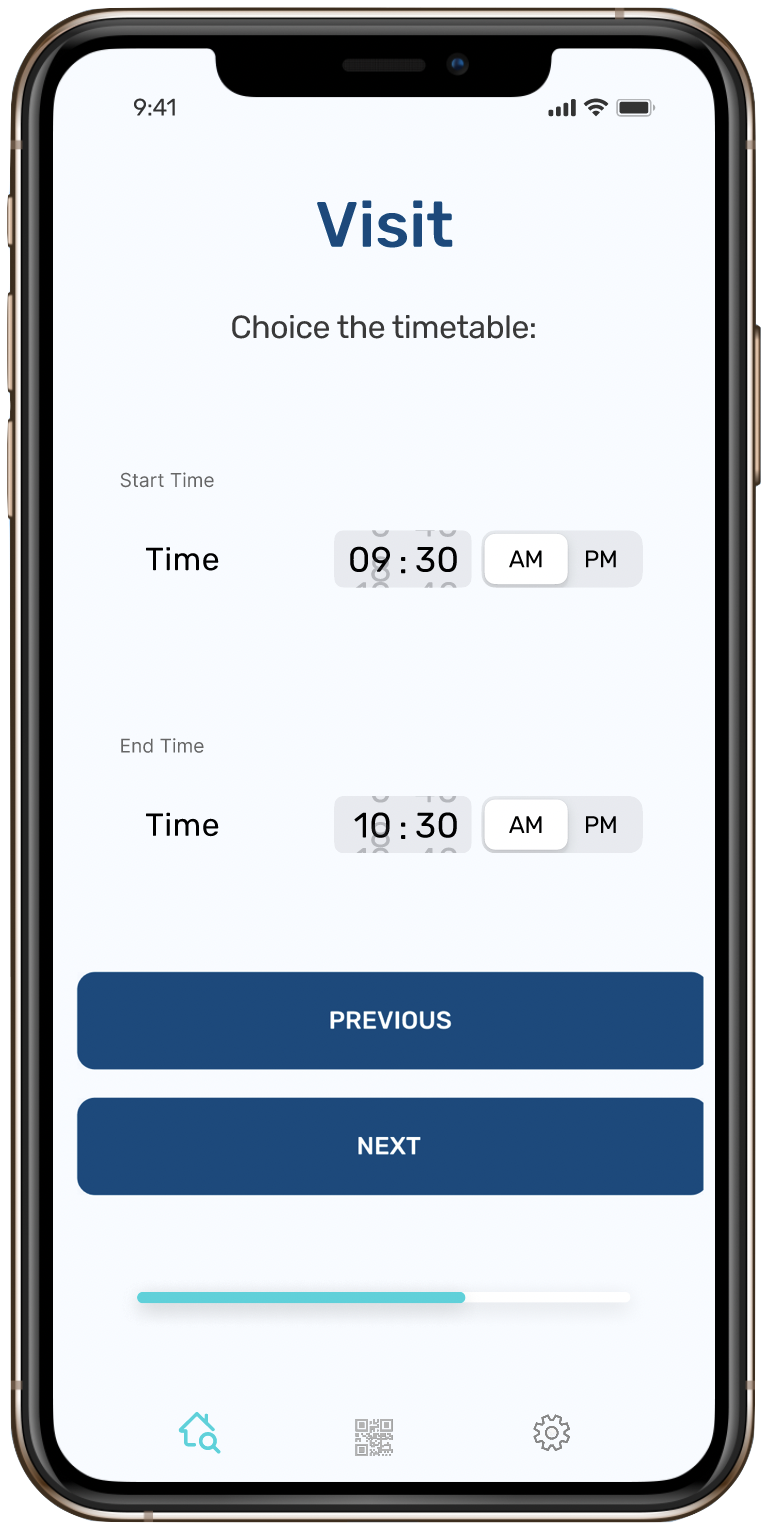
\includegraphics[scale=0.35]{images/mockup/visit2.png}
        }\\ %  ------- End of the first row ----------------------%
        \subfloat[Caption of Third Figure]{%
            \label{fig:third}
            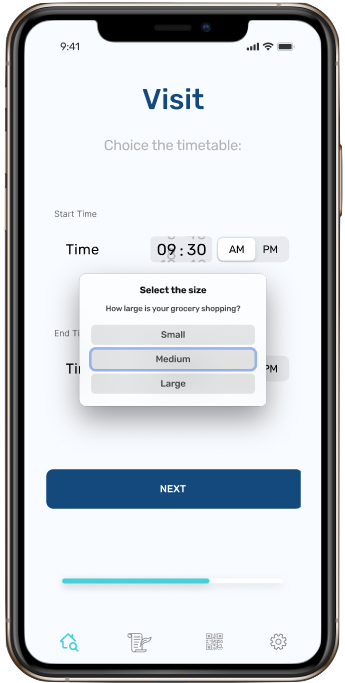
\includegraphics[scale=0.35]{images/mockup/visit_size.png}
        }%
        \subfloat[Caption of Fourth Figure]{%
            \label{fig:fourth}
            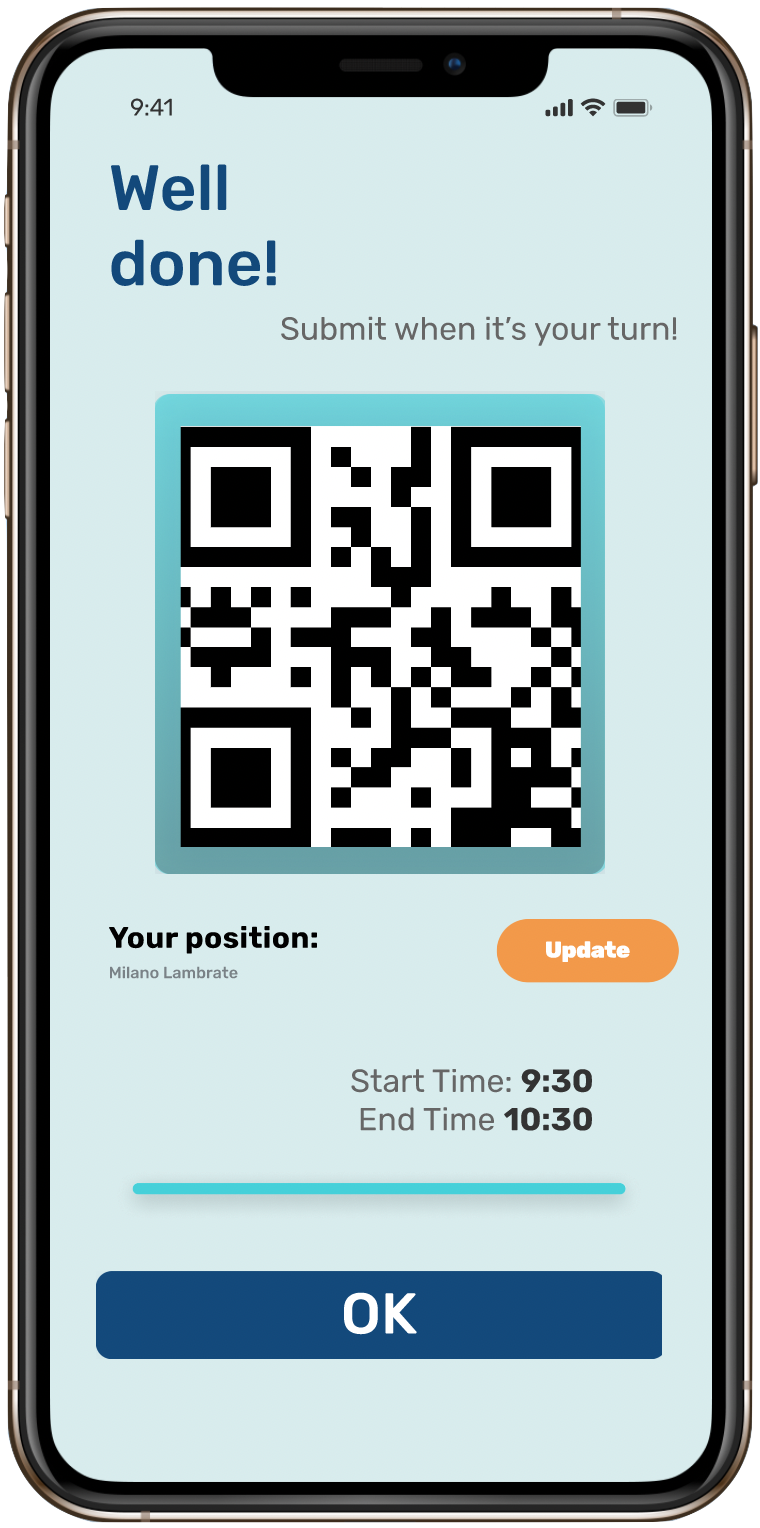
\includegraphics[scale=0.35]{images/mockup/qr_visit_done.png}
        }%
%
    \end{center}
    \caption{%
        The l-o-n-g caption for all the subfigures
        (FirstFigure through FourthFigure) goes here.
     }%
   \label{fig:subfigures}
\end{figure}



\begin{figure}[ht!]
     \begin{center}
%
        \subfloat[Caption of First Figure]{%
            \label{fig:first}
            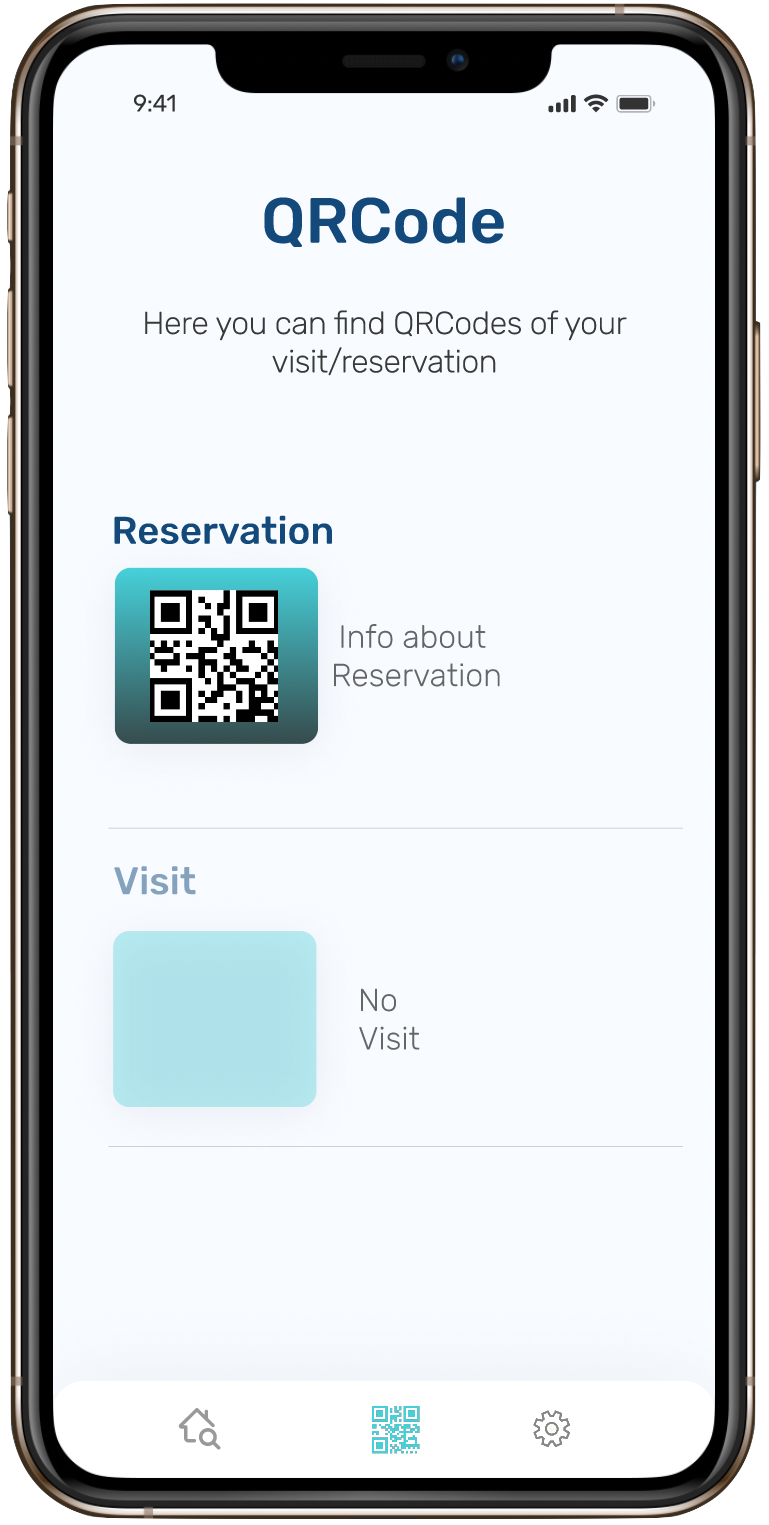
\includegraphics[scale=0.35]{images/mockup/qr2.png}
        }%
        \subfloat[Caption of Second Figure]{%
           \label{fig:second}
           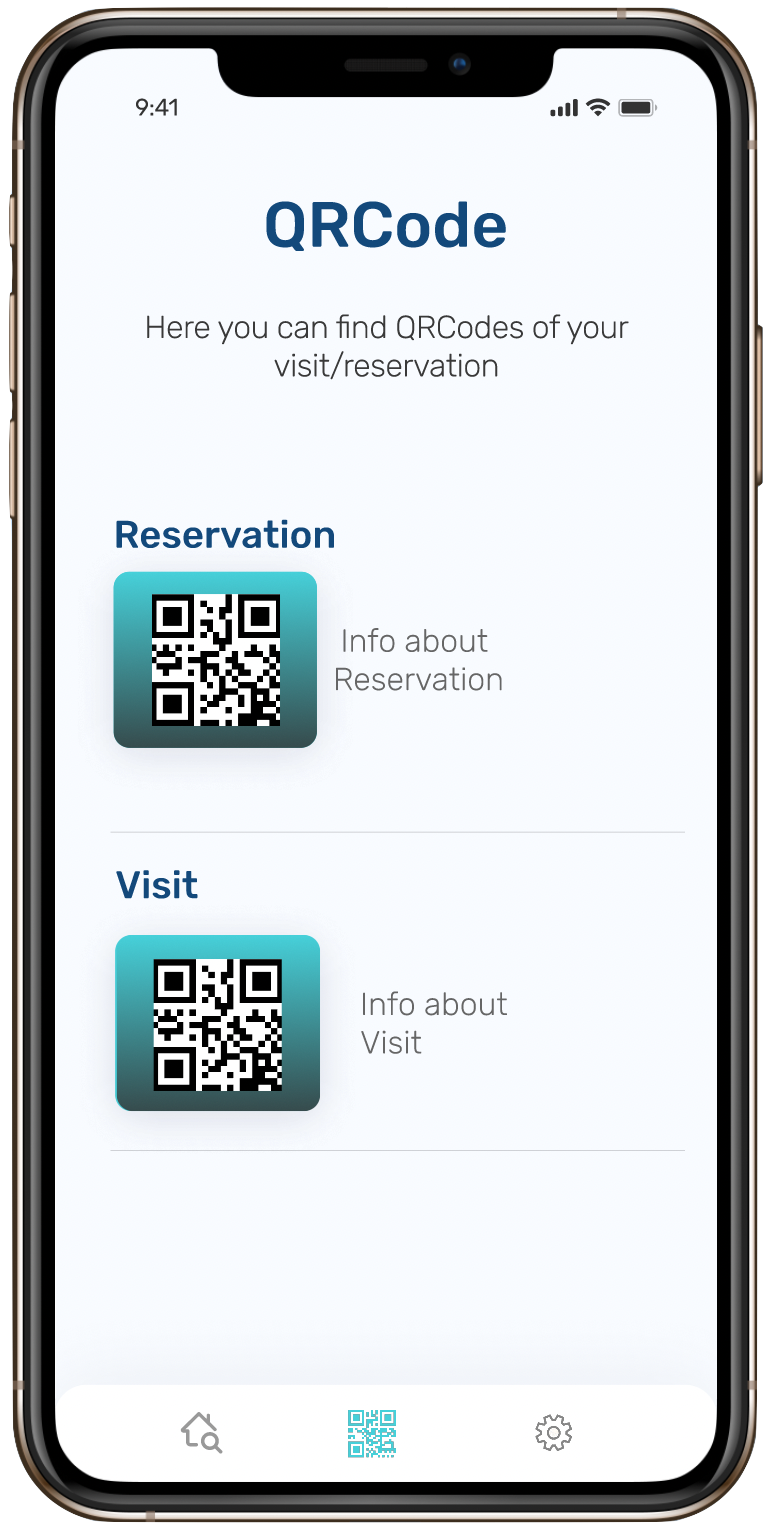
\includegraphics[scale=0.35]{images/mockup/qr4.png}
        }\\ %  ------- End of the first row ----------------------%
        \subfloat[Caption of Third Figure]{%
            \label{fig:third}
            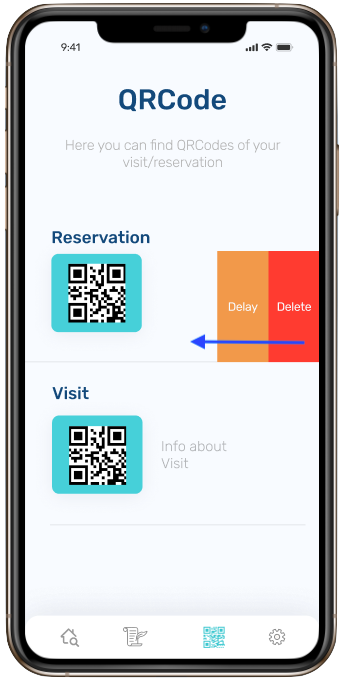
\includegraphics[scale=0.35]{images/mockup/qr5.png}
        }%
        \subfloat[Caption of Fourth Figure]{%
            \label{fig:fourth}
            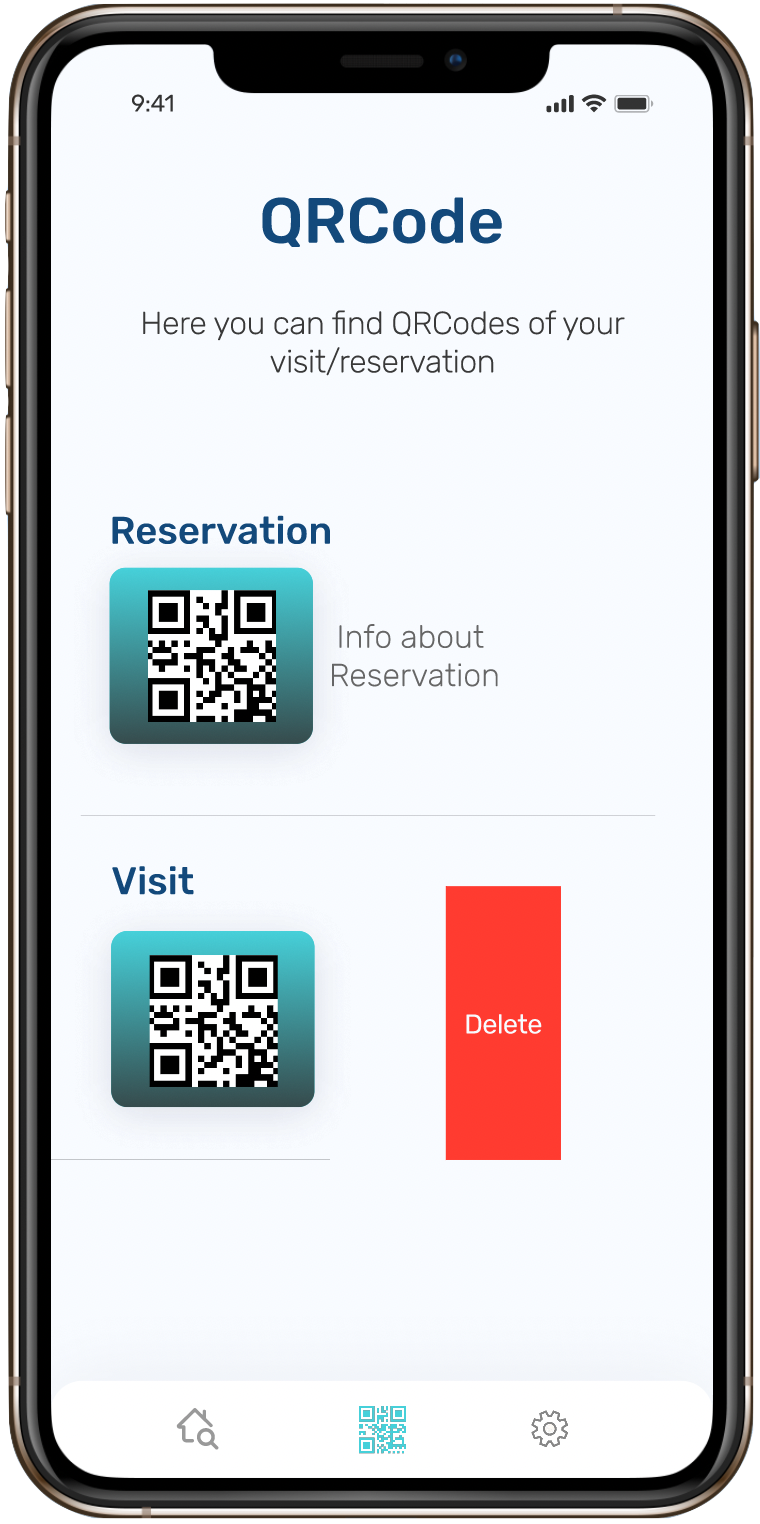
\includegraphics[scale=0.35]{images/mockup/qr6.png}
        }%
%
    \end{center}
    \caption{%
        The l-o-n-g caption for all the subfigures
        (FirstFigure through FourthFigure) goes here.
     }%
   \label{fig:subfigures}
\end{figure}


\begin{figure}[!tbp]
  \centering
  \subfloat[Flower one.]{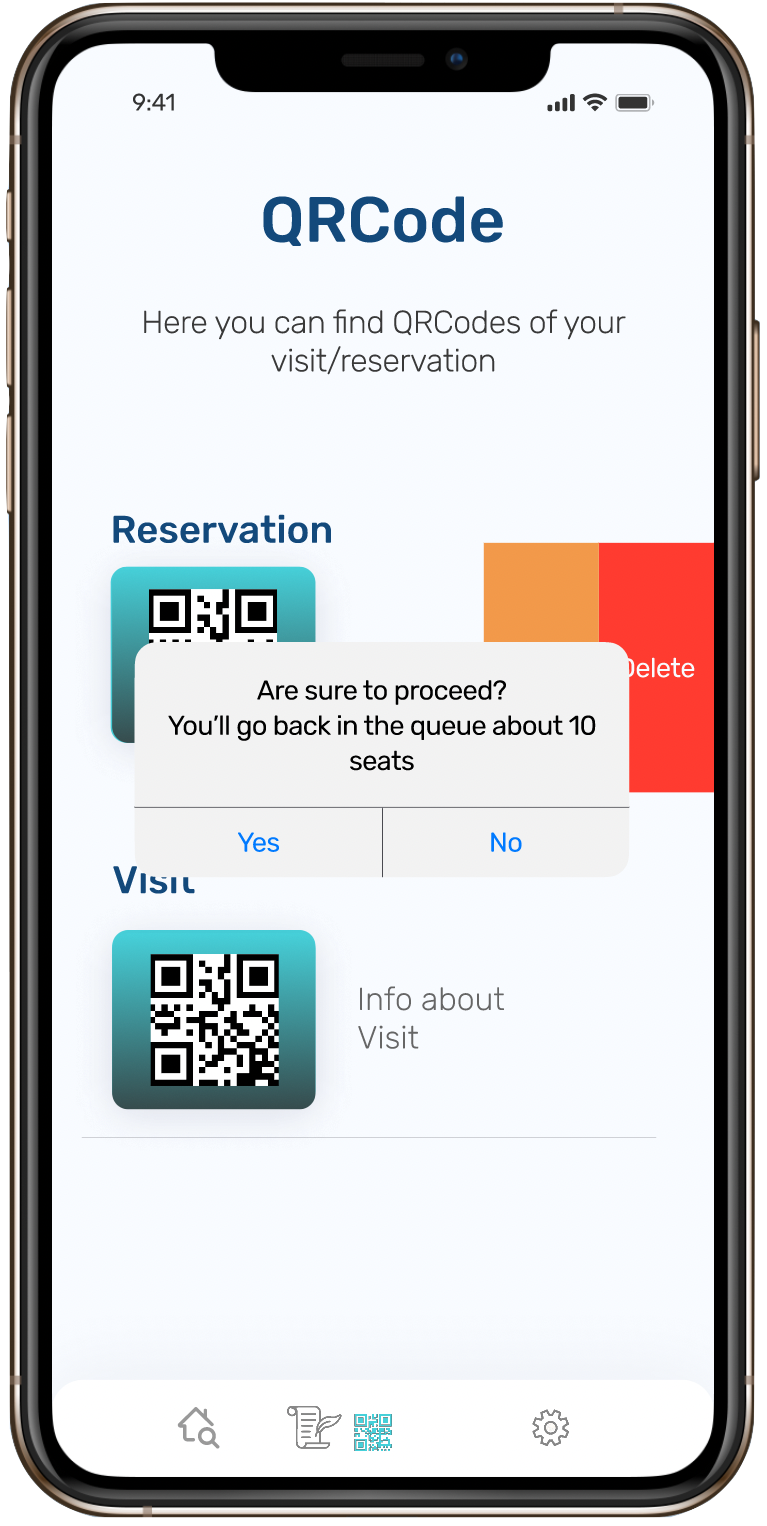
\includegraphics[scale=0.35]{images/mockup/qr1.png}\label{fig:f1}}
  \hfill
  \subfloat[Flower two.]{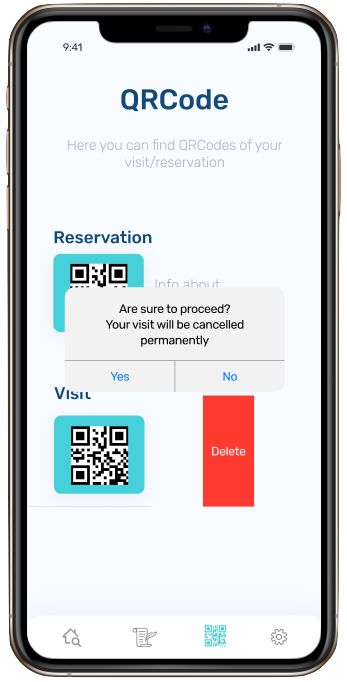
\includegraphics[scale=0.35]{images/mockup/qr7.png}\label{fig:f2}}
  \caption{My flowers.}
\end{figure}



\subsection{Hardware Interfaces}
\subsection{Software Interfaces}
\subsection{Communication Interfaces}
\section{Functional Requirements}
Giovanna, a career woman who is always in trouble to find free time, needs to go grocery shopping for her family. 
Indeed, once she finished working, she goes to the market and, due to the lockdown, have to wait in line for hours to have access to it. The result is that, coming back home later, she can't put some time in her children.
However, in the past days, she discovered CLup App which allows her to book a visit in the market in advance, by only putting the range time avaiable and the size of the expenditure.
In this way, Giovanna will save a lot of time and will stay longer with her children, instead of waiting in line outside the market.

Nevertheless, due to Covid-19 emergency, the market will be always filled.

Jonhathan, on the advice of his grandchild, bought a new smartphone.  In addition started using it and installing usefull applications like CLup.
In particular, with it, he'll be able to make a reservation in market's queue. In this way, CLup will notify him when, accordingly to his position, leave to get the market in time for his turn.
Finally, once he arrived, can go in there by simply scanning the QRCode sent before. 
At the end Jonhathan will go shopping without waiting on feet his turn during a cold winter's day.
Gustavo, an elderly person, he discovered recently a new time saver and usefull service at the market. It consists in booking a visit at the market by simply calling the number found in an advertisment. 
Due to the fact that Gustavo is sick of waiting too much in the queue, decides to call this market number to book the visit.
On the other side Marta, a gentle receptionist who works for the market, answers to Gustavo's call; she takes care of the registration of his own data, the credentials and the all visit information (i.e data and range time).

Gustavo will be notified about the appointment with an SMS on his mobilephone in time. In addition the SMS will provide the schedule for the visit and the code which will be submitted at the entrance.

\begin{figure}[h]
	\caption{Use case USER}
	\label{fig:UML}
	
	\centering
	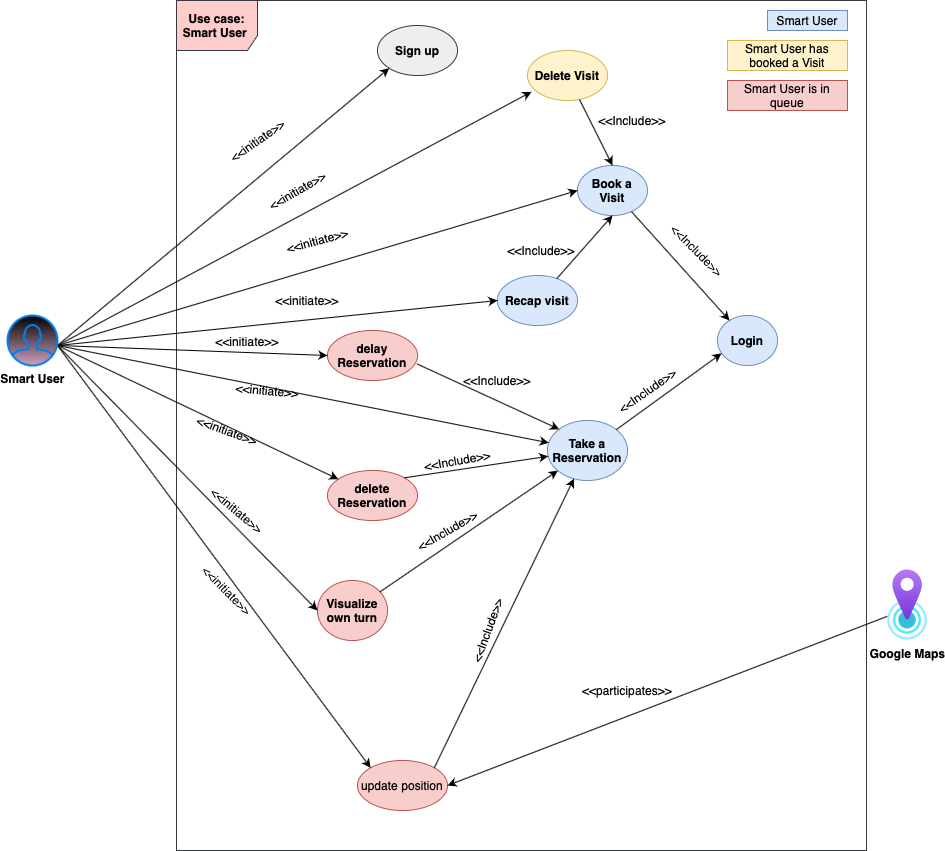
\includegraphics[width=1\textwidth, height=1\textwidth]{diagrams/UseCaseUser.png}
	
\end{figure}

\addvspace{1cm} 
{\normalsize \textbf{Use cases}}
\par \medskip

\begin{tabular}{|p{5cm} | p{7cm} | }
\hline
Name & Login \\
\hline
Actor & User \\
\hline
Entry condition &
\begin{itemize}
\item The user has register
\item The user opened the application
\end{itemize} \\
\hline
Events flow & 
\begin{itemize}
	\item The user open the application
	\item Enters username and password
	\item Click “Login button”
\end{itemize} \\
\hline
Exit condition & User log in \\
\hline 
Exceptions &
\begin{itemize}
	\item User enters wrong username
	\item User enters wrong password
\end{itemize} \\
\hline
\end{tabular}

\par \medskip

\begin{tabular}{|p{5cm} | p{7cm} | }
	\hline
	Name & Sign up \\
	\hline
	Actor & User \\
	\hline
	Entry condition &
	\begin{itemize}
		\item User enters for the first time on the app 
		\item The user hasn’t registered
	\end{itemize} \\
	\hline
	Events flow & 
	\begin{itemize}
		\item The user selects “Create new account” option
		\item The user enters required fields
		\item The user accepts CLup privacy policy
		\item The user clicks “Register” button
	\end{itemize} \\
	\hline
	Exit condition & The users is registered \\
	\hline 
	Exceptions &
	\begin{itemize}
		\item The users has already been registered
		\item The user did not accept CLup privacy policy
		\item The user enters username that has already been used
		\item The user enters prohibited characters
	\end{itemize} \\
	\hline
\end{tabular}

\par \medskip

\begin{tabular}{|p{5cm} | p{7cm} | }
	\hline
	Name & Book a visit \\
	\hline
	Actor & User \\
	\hline
	Entry condition &
	\begin{itemize}
		\item The user has logged in 
	\end{itemize} \\
	\hline
	Events flow & 
	\begin{itemize}
		\item The user click on Home Page
		\item Click on “Book a visit” button
		\item Select the visit date
		\item Select the visit time
		\item Insert shopping size
		\item Click on “Next” button
	\end{itemize} \\
	\hline
	Exit condition & The user book a visit \\
	\hline 
	Exceptions & \\
	\hline
\end{tabular}

\par \medskip

\begin{tabular}{|p{5cm} | p{7cm} | }
	\hline
	Name & Take reservation \\
	\hline
	Actor & User \\
	\hline
	Entry condition &
	\begin{itemize}
		\item The user has logged in 
	\end{itemize} \\
	\hline
	Events flow & 
	\begin{itemize}
		\item The user click on “Home Page” menù
		\item Click on “Reserve a seat” button
		\item Confirm the reservation
	\end{itemize} \\
	\hline
	Exit condition &
	\begin{itemize}	
		\item The user has been queued
		\item The QR code has been associated with user 
	\end{itemize} \\
	\hline 
	Exceptions & The shop is closed \\
	\hline
\end{tabular}

\par \medskip

\begin{tabular}{|p{5cm} | p{7cm} | }
	\hline
	Name & Delete Visit \\
	\hline
	Actor & UserVisiting \\
	\hline
	Entry condition &
	\begin{itemize}
		\item The user has logged in
		\item The user took a visit
	\end{itemize} \\
	\hline
	Events flow & 
	\begin{itemize}
		\item The user clicks on “QR code” menù
		\item The visits and reservation are listed
		\item The user clicks on “Delete” button near the visit
		\item The user confirms the cancellation
	\end{itemize} \\
	\hline
	Exit condition &
	\begin{itemize}	
		\item The system delete user visit
		\item The system make available date and time of user visit
	\end{itemize} \\
	\hline 
	Exceptions & \\
	\hline
\end{tabular}

\par \medskip

\begin{tabular}{|p{5cm} | p{7cm} | }
	\hline
	Name & Delete reservation \\
	\hline
	Actor & UserInQueue \\
	\hline
	Entry condition &
	\begin{itemize}
		\item The user has logged in
		\item The user took a reservation
	\end{itemize} \\
	\hline
	Events flow & 
	\begin{itemize}
		\item The user clicks on “QR code” menù
		\item The visits and reservation are listed
		\item The user clicks on “Delete” button near the reservation
		\item The user confirms the cancellation
	\end{itemize} \\
	\hline
	Exit condition &
	The system delete user reservation \\
	\hline 
	Exceptions & \\
	\hline
\end{tabular}

\par \medskip

\begin{tabular}{|p{5cm} | p{7cm} | }
	\hline
	Name & Delay reservation \\
	\hline
	Actor & UserInQueue \\
	\hline
	Entry condition &
	\begin{itemize}
		\item The user has logged in
		\item The user took a reservation
	\end{itemize} \\
	\hline
	Events flow & 
	\begin{itemize}
		\item The user clicks on “QR code” menù
		\item The visits and reservation are listed
		\item The user clicks on “Delay” button near the reservation
		\item The user confirms the delay
	\end{itemize} \\
	\hline
	Exit condition &
	\begin{itemize}
		\item The user turn will be shift ten places after.
		\item The delay button will be disabled.
	\end{itemize} \\
	\hline 
	Exceptions & 
	\begin{itemize}
		\item The user queue is too small
		\item The user delay function has already been used
	\end{itemize} \\
	\hline
\end{tabular}

\par \medskip

\begin{tabular}{|p{5cm} | p{7cm} | }
	\hline
	Name & Recap visit \\
	\hline
	Actor & User \\
	\hline
	Entry condition &
	The user has logged in \\
	\hline
	Events flow & 
	The user click on “history” menù \\
	\hline
	Exit condition &
	The visits and reservation are listed \\
	\hline 
	Exceptions & \\
	\hline
\end{tabular}

\par \medskip

\begin{tabular}{|p{5cm} | p{7cm} | }
	\hline
	Name & Visualize own turn \\
	\hline
	Actor & UserInQueue \\
	\hline
	Entry condition &
	\begin{itemize}
		\item The user has logged in
		\item The user took a reservation
	\end{itemize} \\
	\hline
	Events flow & 
	The user clicks on “history” menù \\
	\hline
	Exit condition &
	The system show the user turn near the reservation QR code \\
	\hline 
	Exceptions & \\
	\hline
\end{tabular}

\par \medskip

\begin{tabular}{|p{5cm} | p{7cm} | }
	\hline
	Name & Update position  \\
	\hline
	Actor & UserInQueue \\
	\hline
	Entry condition &
	\begin{itemize}
		\item The user has logged in
		\item The user took a reservation
	\end{itemize} \\
	\hline
	Events flow & 
	\begin{itemize}
		\item The user clicks on “QR code” menù
		\item The user clicks on “Update position”
	\end{itemize} \\
	\hline
	Exit condition &
	The system calculate the number of customers in queue after which will send the message  \\
	\hline 
	Exceptions & 
	\begin{itemize}
		\item GPS position too far from supermarket
		\item Invalid GPS position
		\item GPS is inactive
	\end{itemize} \\
	\hline
\end{tabular}

\par \medskip

\begin{tabular}{|p{5cm} | p{7cm} | }
	\hline
	Name & Choice market  \\
	\hline
	Actor & User \\
	\hline
	Entry condition &
	User login for the first time on the app \\
	\hline
	Events flow & 
	\begin{itemize}
		\item Select the supermarket
		\item Click “Next” to confirm
	\end{itemize} \\
	\hline
	Exit condition &
	The system calculate the number of customers in queue after which will send the message  \\
	\hline 
	Exceptions & 
	The user is linked to supermarket \\
	\hline
\end{tabular}

\par \medskip

\subsection{Reception}
\par \medskip
{\large \textbf{Scenarios}}
\par \medskip
{\normalsize \textbf{Scenario 1}}
\par \medskip
 Gustavo, an elderly person, he discovered recently a new time saver and usefull service at the market. \\
 It consists to book a visit at the market by simply calling the number found in an advertisment. \\
 Due to the fact that Gustavo is sick of waiting too much in the queue decide to call this market number to book the visit. \\
 On the other side Marta, a gentle receptionist who works for the market, answers to Gustavo's call; she takes care of the registration of his own data, the credentials and the all visit information (i.e data and range time).\\
  Gustavo will be notified about the appointment with an SMS on his mobilephone in time. \\
  In addition the SMS will provide the schedule for the visit and the code which will be submitted at the entrance.
 
 \par \medskip 
 
 \begin{figure}[h]
 	\caption{Use case RECEPTION}
 	\label{fig:UML}
 	
 	\centering
 	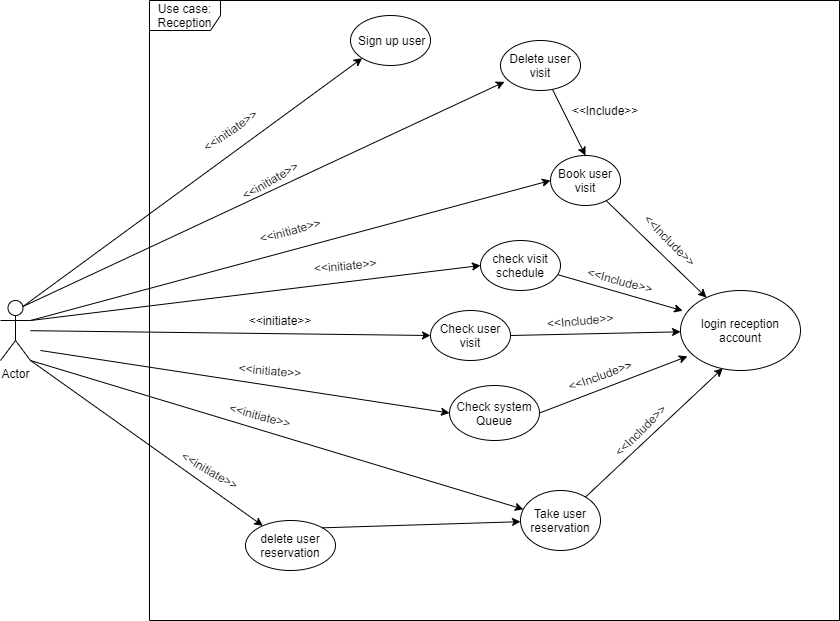
\includegraphics[width=1\textwidth, height=1\textwidth]{diagrams/UseCaseReception.png}
 	
 \end{figure}
 
 \addvspace{1cm} 
 {\normalsize \textbf{Use cases}}
 \par \medskip
 
 \begin{tabular}{|p{5cm} | p{7cm} | }
 	\hline
 	Name & Sign up user  \\
 	\hline
 	Actor & Reception \\
 	\hline
 	Entry condition &
 	\begin{itemize}
 		\item The receptionist has logged in 
 		\item The user has not registered
 	\end{itemize} \\
 	\hline
 	Events flow & 
 	\begin{itemize}
 		\item The receptionist asks required information to do registration
 		\item The receptionist fills the fields
 		\item The receptionist confirms the registration
 	\end{itemize} \\
 	\hline
 	Exit condition &
 	The user has registered \\
 	\hline 
 	Exceptions & 
 	\begin{itemize}
 		\item The phone cuts out
 		\item The user has already registered
 	\end{itemize} \\
 	\hline
 \end{tabular}

\begin{tabular}{|p{5cm} | p{7cm} | }
	\hline
	Name & Delete user visit  \\
	\hline
	Actor & Reception \\
	\hline
	Entry condition &
	\begin{itemize}
		\item The receptionist has logged in 
		\item The user wants delete a visit
	\end{itemize} \\
	\hline
	Events flow & 
	\begin{itemize}
		\item The receptionist asks user information
		\item The receptionist asks visit information
		\item The receptionist checks the visit on the menù
		\item Delete user visit clicking “delete” button
	\end{itemize} \\
	\hline
	Exit condition &
	The user visit is deleted\\
	\hline 
	Exceptions & 
	The user has not booked any visits \\
	\hline
\end{tabular}

\begin{tabular}{|p{5cm} | p{7cm} | }
	\hline
	Name & Book user visit  \\
	\hline
	Actor & Reception \\
	\hline
	Entry condition &
	\begin{itemize}
		\item The receptionist has logged in 
		\item The user must be registered
	\end{itemize} \\
	\hline
	Events flow & 
	\begin{itemize}
		\item The receptionist asks the credentials
		\item The receptionist enters the credentials in the system to check registration
		\item Click “select” button on user row
		\item Click “book a visit” button 
		\item The receptionist check free slot and agree with user date and time
		\item Enter date,start time, end time
		\item The receptionist confirms the visit
	\end{itemize} \\
	\hline
	Exit condition &
	The user book a visit\\
	\hline 
	Exceptions & 
	The phone cuts out \\
	\hline
\end{tabular}
 
 \begin{tabular}{|p{5cm} | p{7cm} | }
 	\hline
 	Name & Check user visit  \\
 	\hline
 	Actor & Reception \\
 	\hline
 	Entry condition &
 	\begin{itemize}
 		\item The receptionist has logged in 
 		\item The user must be registered
 	\end{itemize} \\
 	\hline
 	Events flow & 
 	\begin{itemize}
 		\item The receptionist check user registration
 		\item The receptionist check user visits
 	\end{itemize} \\
 	\hline
 	Exit condition &
 	The system list all user visits \\
 	\hline 
 	Exceptions & 
 	\begin{itemize}
 		\item The user does not exist
 		\item The user has not booked any visits
 	\end{itemize} \\
 	\hline
 \end{tabular}


\begin{tabular}{|p{5cm} | p{7cm} | }
	\hline
	Name & Check visit schedule \\
	\hline
	Actor & Reception \\
	\hline
	Entry condition & 
	The receptionist has logged in \\
	\hline
	Events flow & 
	\begin{itemize}
		\item The receptionist click on calendar
		\item The system lists all free dates
		\item The receptionist click on date
	\end{itemize} \\
	\hline
	Exit condition &
	The system lists all date free slot \\
	\hline 
	Exceptions & \\
	\hline
\end{tabular}

\begin{tabular}{|p{5cm} | p{7cm} | }
	\hline
	Name & Check system queue \\
	\hline
	Actor & Reception \\
	\hline
	Entry condition & 
	The receptionist has logged in  \\
	\hline
	Events flow & 
	The receptionist clicks on “Check queue”  \\
	\hline
	Exit condition &
	The system lists all user in queue information \\
	\hline 
	Exceptions & The queue is empty \\
	\hline
\end{tabular}

\begin{tabular}{|p{5cm} | p{7cm} | }
	\hline
	Name & Take user reservation \\
	\hline
	Actor & Reception \\
	\hline
	Entry condition &
	\begin{itemize}
		\item The receptionist has logged in 
		\item The user must be registered
	\end{itemize} \\
	\hline
	Events flow & 
	\begin{itemize}
		\item The receptionist asks the credentials
		\item The receptionist enters the credentials in the system to check registration
		\item Click “select” button on user row
		\item Click “reserve a sit” button 
		\item The receptionist confirms the reservation
	\end{itemize} \\
	\hline
	Exit condition &
	The user has been queued \\
	\hline 
	Exceptions & 
	The queue is full \\
	\hline
\end{tabular}

\begin{tabular}{|p{5cm} | p{7cm} | }
	\hline
	Name & Delete user reservation \\
	\hline
	Actor & Reception \\
	\hline
	Entry condition &
	\begin{itemize}
		\item The receptionist has logged in 
		\item The user must be registered
	\end{itemize} \\
	\hline
	Events flow & 
	\begin{itemize}
		\item The receptionist asks user information
		\item The receptionist checks the reservation on the menù
		\item Delete user reservation clicking “delete” button
	\end{itemize} \\
	\hline
	Exit condition &
	The user reservation is deleted \\
	\hline 
	Exceptions & 
	The user has not booked any reservation \\
	\hline
\end{tabular}

\begin{tabular}{|p{5cm} | p{7cm} | }
	\hline
	Name & Login reception account \\
	\hline
	Actor & Reception \\
	\hline
	Entry condition &
	The receptionist open desktop app  \\
	\hline
	Events flow & 
	\begin{itemize}
		\item The receptionist enter the credentials to log in 
		\item Click on “Sign in” button
	\end{itemize} \\
	\hline
	Exit condition &
	The receptionist has logged in \\
	\hline 
	Exceptions & 
	\begin{itemize}
		\item Wrong password
		\item Wrong username
	\end{itemize} \\
	\hline
\end{tabular}


\section{Performance Requirements}
\section{Design Constraints}
\subsection{Standards compliance}
Especially, the system will be released in the main digital distribution platform (such as App Store or Google Play). So it must follow their guidelines in order to have a proper and a lawful distribution. In addition, due to the fact that it retrives and analyses many sensitive data, application must respect tha main privacy guidance. In particular in Europe must follow the General Data Privacy Regulation (GDPR), due to a safe and aware processing of data. 
\subsection{Hardware limitations}
\begin{itemize}
\item 2G/3G/4G/5G connection: they're essential due to server connection to compile booking request;
\item GPS: it's used to allow user to estimate the time spending to reach the market in time. But it's not mandatory for booking;
\end{itemize}
\subsection{Any other constraint}
There are no other constraint.
\section{Software System Attributes}
\subsection{Reliability}
The application have to provide user the possibility to book both reservation and visit successfully. [TODO] 
\subsection{Availability}
Due to the fact that nowadays grocery shopping is avaiable almost all day, the availability of the system is very high. So the required availability is close to 99\%. However, the reservation function has a lower avaibility because of the inability to book a seat in queue if the market is closed in some hours of the day. 
\subsection{Security}
Security is one of the most critical aspect of CLup. So User's sensitive data are stored safely DBMS accessibile only by strict level of privilege. In addition, communication towards the application server (like login or booking requests) are implemented using  HTTPS protocol, which, with TLS protocol, ensure the encryption of every packets. 
\subsection{Maintainability}
The application implementation must be oriented towards an high scalability in order to gurantee an efficient and cheaper maintenance. This could be done by using design patterns.
\subsection{Portability}
The system must be smoothly portable almost the main smartphone on the market. So CLup must be distributed for the main mobile operating system (i.e App Store and Google Play), coding it with program language such as Android or Swing. In addition CLup Guest, the application used by receptionist to book visit and reservation of the Users not register, must be compatible with the main Operating system such as Windows and Mac OS X. [todo]